\documentclass[tikz,border=8pt]{standalone}
% Shared look for every TikZ diagram. Load with % Shared look for every TikZ diagram. Load with % Shared look for every TikZ diagram. Load with \input{../../tools/tikz-style.tex}
\usepackage[T1]{fontenc}
\usepackage{lmodern}
\renewcommand{\sfdefault}{lmr}  % diagrams use the same serif as the text
\usetikzlibrary{arrows.meta, positioning, shapes.geometric, calc, fit, backgrounds}
\definecolor{cblue}{HTML}{4C78A8}
\definecolor{corange}{HTML}{F58518}
\definecolor{cgreen}{HTML}{54A24B}
\definecolor{cred}{HTML}{E45756}
\definecolor{cpurple}{HTML}{B279A2}
\definecolor{cgrey}{HTML}{6B6B6B}
\tikzset{
  every picture/.style={font=\sffamily, line width=1.2pt},
  box/.style={draw=#1, fill=#1!12, rounded corners=4pt, align=center, inner sep=7pt, minimum height=1.1cm},
  box/.default=cgrey,
  arrow/.style={-{Stealth[length=3mm]}, draw=cgrey, line width=1.4pt},
  title/.style={font=\sffamily\bfseries\Large},
  note/.style={font=\sffamily\small, text=cgrey, align=center},
}
\AtBeginDocument{\hyphenpenalty=10000 \exhyphenpenalty=10000}

\usepackage[T1]{fontenc}
\usepackage{lmodern}
\renewcommand{\sfdefault}{lmr}  % diagrams use the same serif as the text
\usetikzlibrary{arrows.meta, positioning, shapes.geometric, calc, fit, backgrounds}
\definecolor{cblue}{HTML}{4C78A8}
\definecolor{corange}{HTML}{F58518}
\definecolor{cgreen}{HTML}{54A24B}
\definecolor{cred}{HTML}{E45756}
\definecolor{cpurple}{HTML}{B279A2}
\definecolor{cgrey}{HTML}{6B6B6B}
\tikzset{
  every picture/.style={font=\sffamily, line width=1.2pt},
  box/.style={draw=#1, fill=#1!12, rounded corners=4pt, align=center, inner sep=7pt, minimum height=1.1cm},
  box/.default=cgrey,
  arrow/.style={-{Stealth[length=3mm]}, draw=cgrey, line width=1.4pt},
  title/.style={font=\sffamily\bfseries\Large},
  note/.style={font=\sffamily\small, text=cgrey, align=center},
}
\AtBeginDocument{\hyphenpenalty=10000 \exhyphenpenalty=10000}

\usepackage[T1]{fontenc}
\usepackage{lmodern}
\renewcommand{\sfdefault}{lmr}  % diagrams use the same serif as the text
\usetikzlibrary{arrows.meta, positioning, shapes.geometric, calc, fit, backgrounds}
\definecolor{cblue}{HTML}{4C78A8}
\definecolor{corange}{HTML}{F58518}
\definecolor{cgreen}{HTML}{54A24B}
\definecolor{cred}{HTML}{E45756}
\definecolor{cpurple}{HTML}{B279A2}
\definecolor{cgrey}{HTML}{6B6B6B}
\tikzset{
  every picture/.style={font=\sffamily, line width=1.2pt},
  box/.style={draw=#1, fill=#1!12, rounded corners=4pt, align=center, inner sep=7pt, minimum height=1.1cm},
  box/.default=cgrey,
  arrow/.style={-{Stealth[length=3mm]}, draw=cgrey, line width=1.4pt},
  title/.style={font=\sffamily\bfseries\Large},
  note/.style={font=\sffamily\small, text=cgrey, align=center},
}
\AtBeginDocument{\hyphenpenalty=10000 \exhyphenpenalty=10000}

\begin{document}
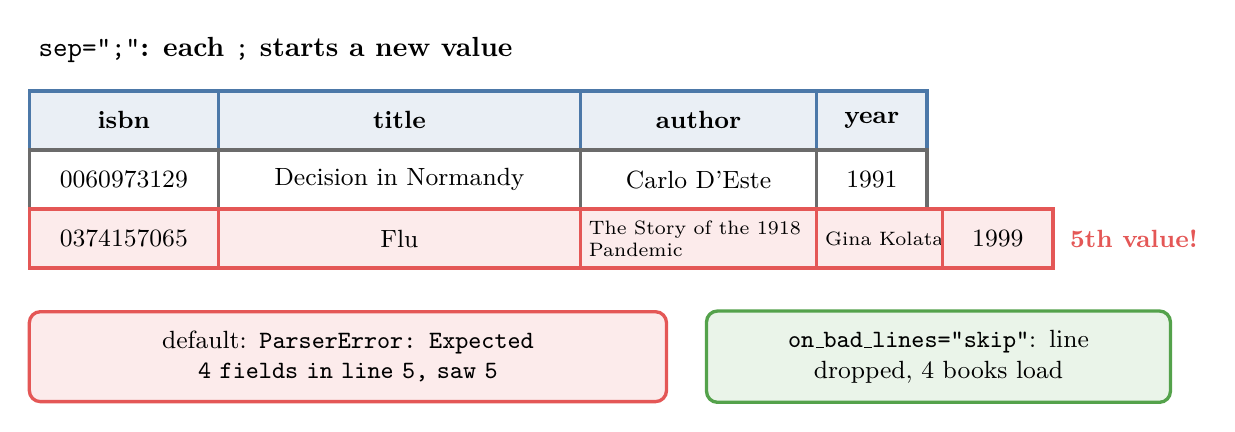
\begin{tikzpicture}[c/.style={draw=#1, fill=#1!12, minimum height=0.75cm, font=\sffamily\small, inner sep=3pt, anchor=west}]
  \node[font=\bfseries, anchor=west] at (0,0.9) {\texttt{sep=";"}: each \texttt{;} starts a new value};
  % header
  \node[c=cblue, minimum width=2.4cm, font=\sffamily\small\bfseries] at (0,0) {isbn};
  \node[c=cblue, minimum width=4.6cm, font=\sffamily\small\bfseries] at (2.4,0) {title};
  \node[c=cblue, minimum width=3.0cm, font=\sffamily\small\bfseries] at (7.0,0) {author};
  \node[c=cblue, minimum width=1.4cm, font=\sffamily\small\bfseries] at (10.0,0) {year};
  % a good line
  \node[c=cgrey, fill=white, minimum width=2.4cm] at (0,-0.75) {0060973129};
  \node[c=cgrey, fill=white, minimum width=4.6cm] at (2.4,-0.75) {Decision in Normandy};
  \node[c=cgrey, fill=white, minimum width=3.0cm] at (7.0,-0.75) {Carlo D'Este};
  \node[c=cgrey, fill=white, minimum width=1.4cm] at (10.0,-0.75) {1991};
  % the bad line
  \node[c=cred, minimum width=2.4cm] at (0,-1.5) {0374157065};
  \node[c=cred, minimum width=4.6cm] at (2.4,-1.5) {Flu};
  \node[c=cred, minimum width=3.0cm, text width=2.8cm, font=\sffamily\scriptsize] at (7.0,-1.5) {The Story of the 1918 Pandemic};
  \node[c=cred, minimum width=1.4cm, font=\sffamily\scriptsize] at (10.0,-1.5) {Gina Kolata};
  \node[c=cred, minimum width=1.4cm, very thick] (x) at (11.6,-1.5) {1999};
  \node[cred, anchor=west, font=\sffamily\small\bfseries] at (13.1,-1.5) {5th value!};
  \node[box=cred, anchor=west, text width=7.6cm, font=\small] at (0,-3.0) {default: \texttt{ParserError: Expected 4 fields in line 5, saw 5}};
  \node[box=cgreen, anchor=west, text width=5.4cm, font=\small] at (8.6,-3.0) {\texttt{on\_bad\_lines="skip"}: line dropped, 4 books load};
\end{tikzpicture}
\end{document}
